\documentclass{article}
\usepackage[utf8]{inputenc}
\usepackage{graphicx}
\usepackage{booktabs}
\usepackage{amsmath, amsthm, amssymb, bm}
\usepackage{tikz, pgfplots}
\usepackage{float}

\title{MA4240 Report}
\author{Dishank, Chirag, Mulugu, Datta}
\date{April 2022}

% What to do
% We will run simulations to verify CLT,
% basically, we will start with a known distribution
% the distributions that we can use are
% uniform, gaussian, cauchy, chi sq, t-distribution
% we will make samples of size 100 for each distribution
% we will make 5000 such samples
% for each sample of size 100, we will find the Xbar.
% CLT states that the distribution of sample means approximates a normal distribution as the sample size gets larger, regardless of the population's distribution.
% Now that we have 1000 values for Xbar, we will make a box plot and histogram and Q-Q plot and then visualise whether or not the distribution of Xbar looks like normal distribution
% note that Xbar will have mean as u (same as original distribution) and variance as sigma/10
%
% Hypothesis Testing
%    Alternate hypothesis
%       CLT is incorrect
%    Null Hypothesis
%       CLT is correct.
% 
% Theory: 
%   type 1 error: rejecting the null hypothesis when it is true (for population parameters)
%   type 2 error: not rejecting the null hypothesis when it is false (for population parameters)
%
% type 2 error is more significant for us here
% because if CLT is actually false, and we are modelling several things assuming it to be True.
%
% The null hypothesis suggests that Xbar follows N(u, sigma*0.1)
% We can make a QQ plot since we know the original normal distribution


\begin{document}
\maketitle

\section{Introduction}
Central Limit Theorem states that normalised sum of independent and identically distributed random variables tends towards a normal distribution, irrespective of the distribution of random variables.
\begin{align}
    Z = \lim_{n \to \infty} \left(\frac{\bar{X}_n-\mu}{\frac{\sigma}{n}}\right) \label{eq:CLT}
\end{align}
In this project, we propose to verify the correctness of Central Limit Theorem by running simulations beginning with a variety of distributions covered in the course.

\section{Central Limit Theorem and imperial approximation}
While equation \eqref{eq:CLT} suggests that $n$ should be a very large number. In practice, we tend to use the theorem for $n>30$. 
\subsection{Proof of CLT}
THE PROOF GOES HERE

\section{Hypothesis}
We formulate our hypothesis in the following manner
\begin{align}
    & H_A\text{ : CLT doesn't hold} \nonumber\\
    & H_0\text{ : CLT holds}\nonumber
\end{align}
Here, type 2 error is when CLT is actually false but we fail to reject it. It is more dangerous because several models are built on the assumption that CLT is indeed correct.
\section{Procedure}
We are generating a batch of $100$ samples from the distribution, we find the sample mean of this batch, call it $\bar{X}$. From Central Limit Theorem, we know
\begin{align}
    \bar{X} \sim \mathcal{N}(\mu, \frac{\sigma^2}{100})
\end{align}
To verify the claim, we repeat this experiment $5000$ times, then perform normality tests, which can be classified into two parts
\begin{enumerate}
    \item Graphical Methods
    \begin{itemize}
        \item Q-Q plot
        \item Histogram
    \end{itemize}
    \item{Frequentist tests}
    \begin{itemize}
        \item Shapiro-wilk test
    \end{itemize}
\end{enumerate}

\subsection{Shapiro-Wilk test}
lorum ipsum dolor sit amet

\subsection{Distributions used}
\begin{enumerate}
    \item \textbf{Standard Normal}: The pdf of standard normal distribution is given by:
    $$f_X(x) = \dfrac{1}{\sqrt{(2\pi)}}exp(-\dfrac{x^2}{2})$$
    The mean is 0 and standard deviation is 1. Figure \ref{normal_pdf} shows the PDF of standard normal distribution.
    \begin{figure}[H]
        \centering
        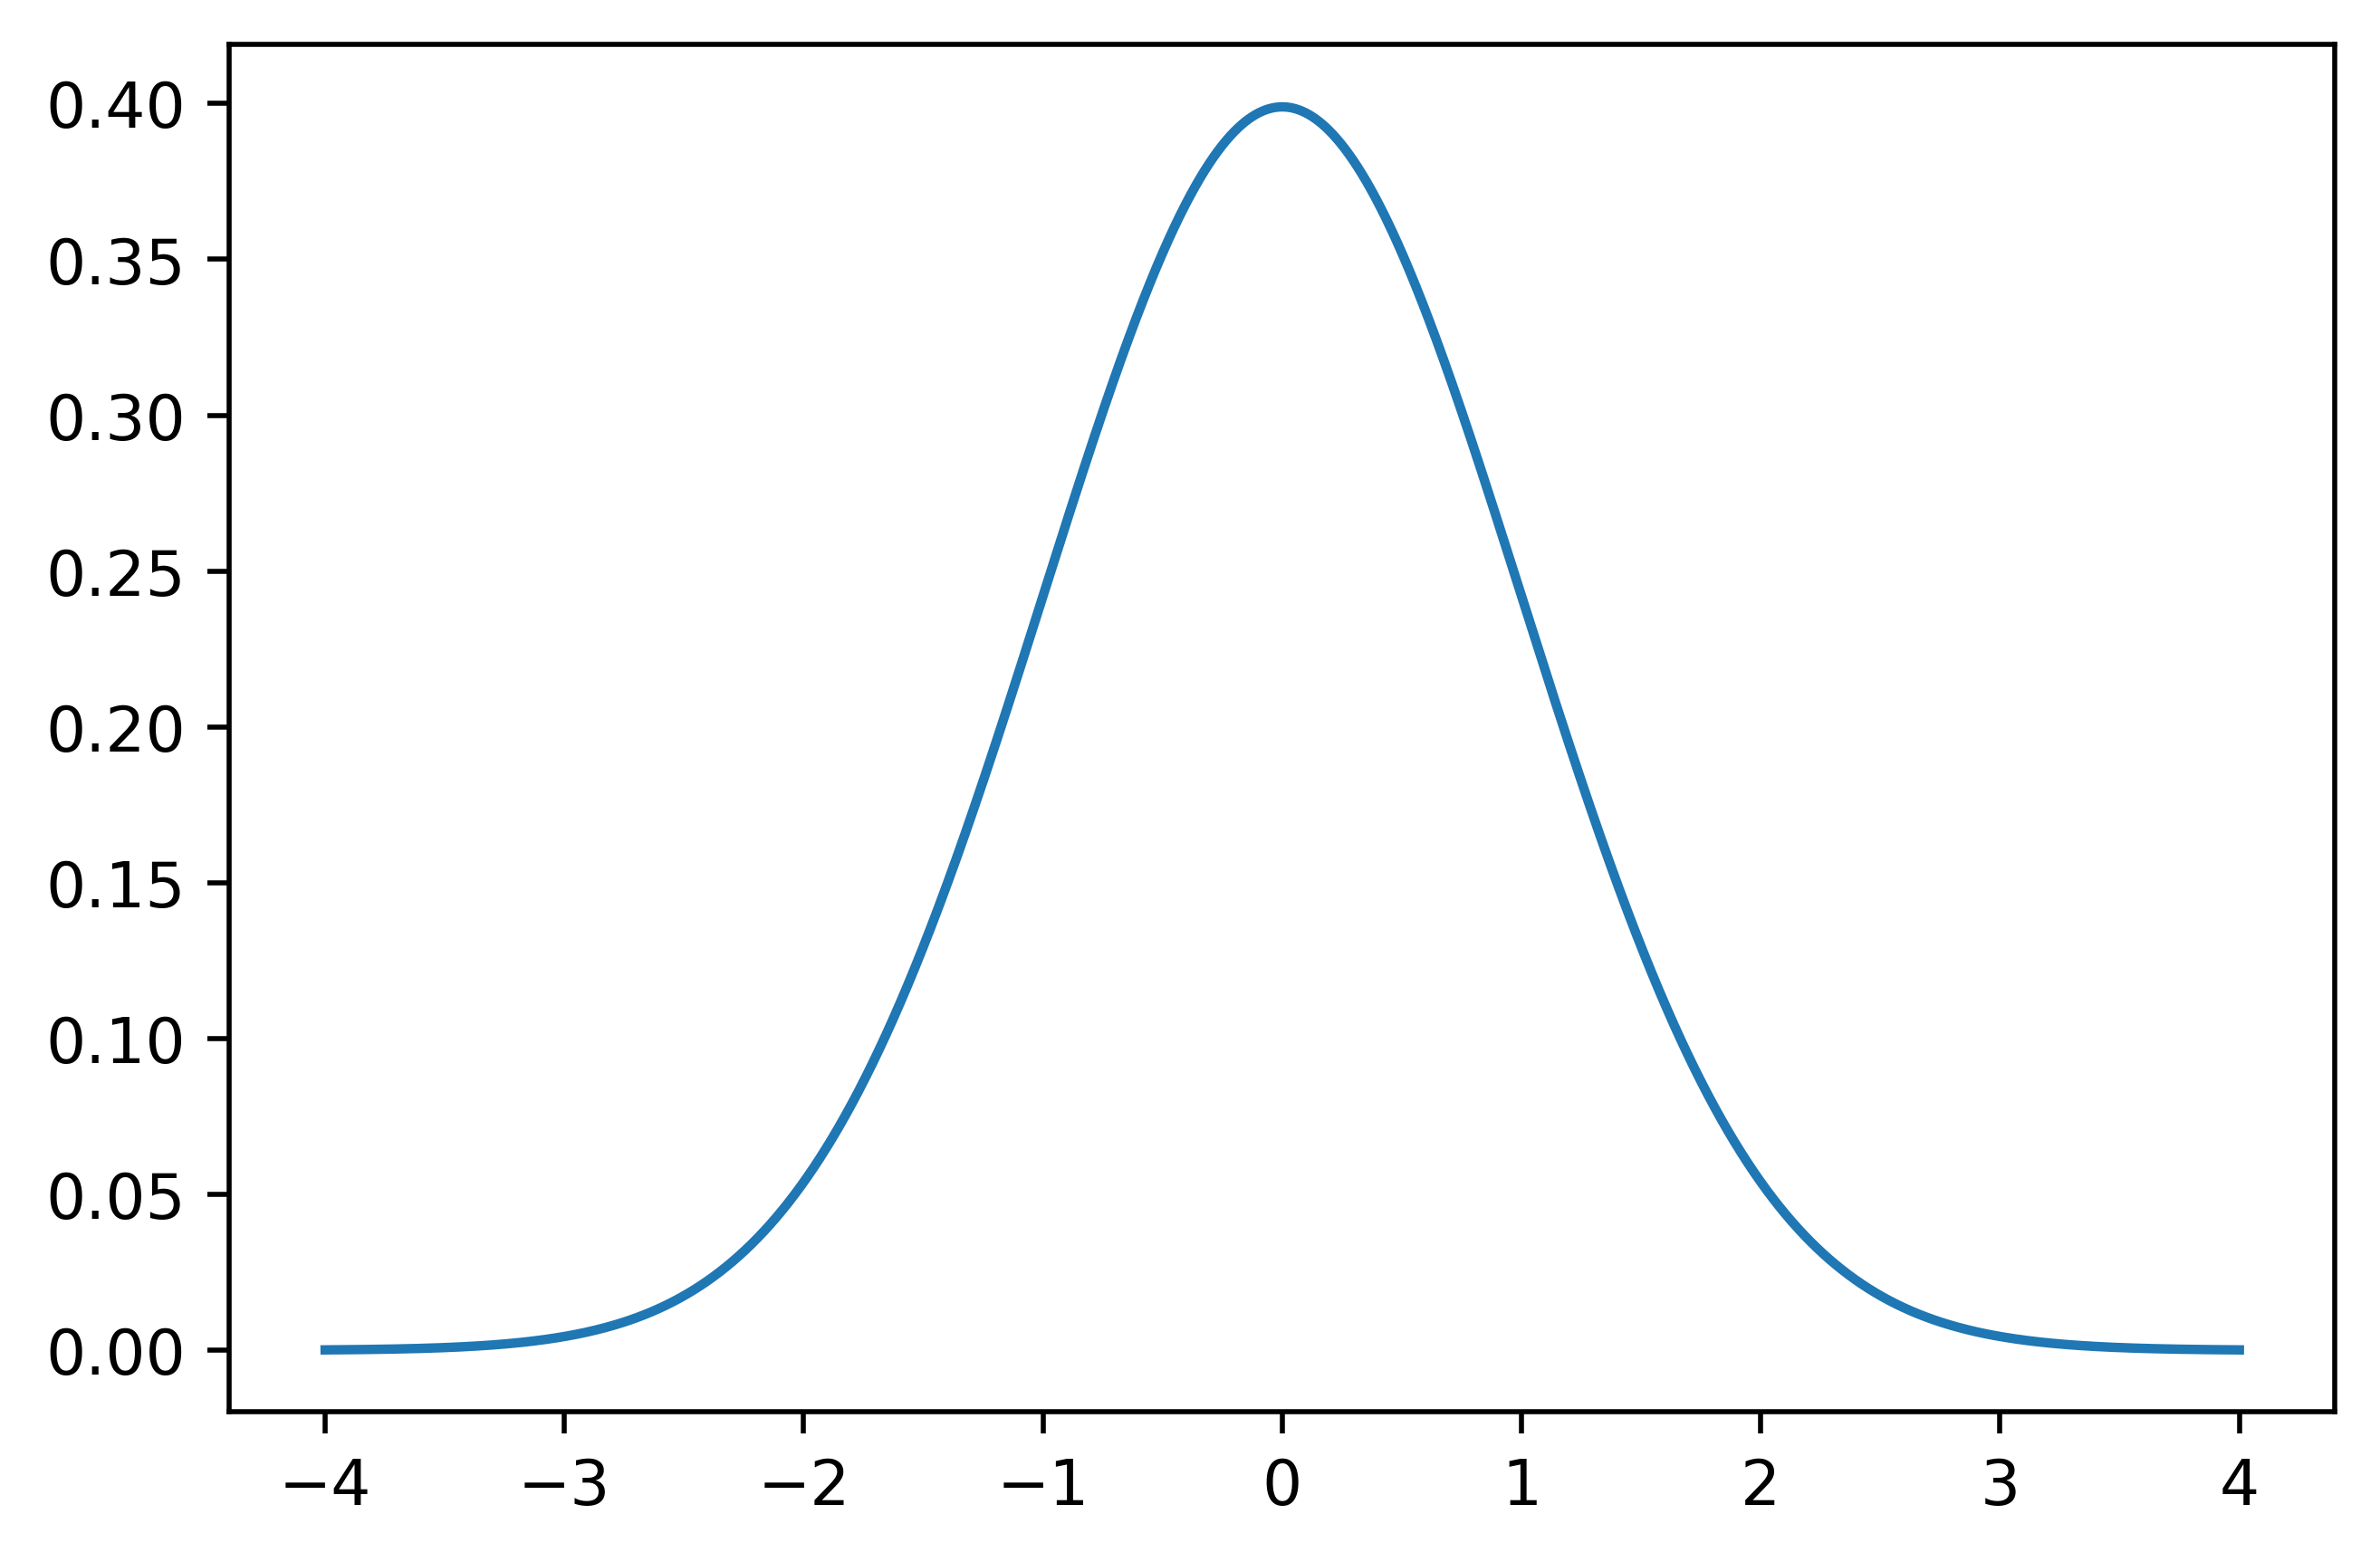
\includegraphics[scale=0.5]{images/gaussian.png}
        \caption{PDF of standard normal distribution}
        \label{normal_pdf}
    \end{figure}
    \item \textbf{Continuous uniform distribution}: Here, we have used U(0, 1). The PMF is given by $$f_X(x) = \begin{cases}1,\; 0 \le x \le 1 \\ 0,\; otherwise\end{cases}$$ 
    The mean is 0.5 and standard deviation is 0.289. Figure \ref{uni_pdf} shows the PDF of the uniform distribution.
    \begin{figure}[H]
        \centering
        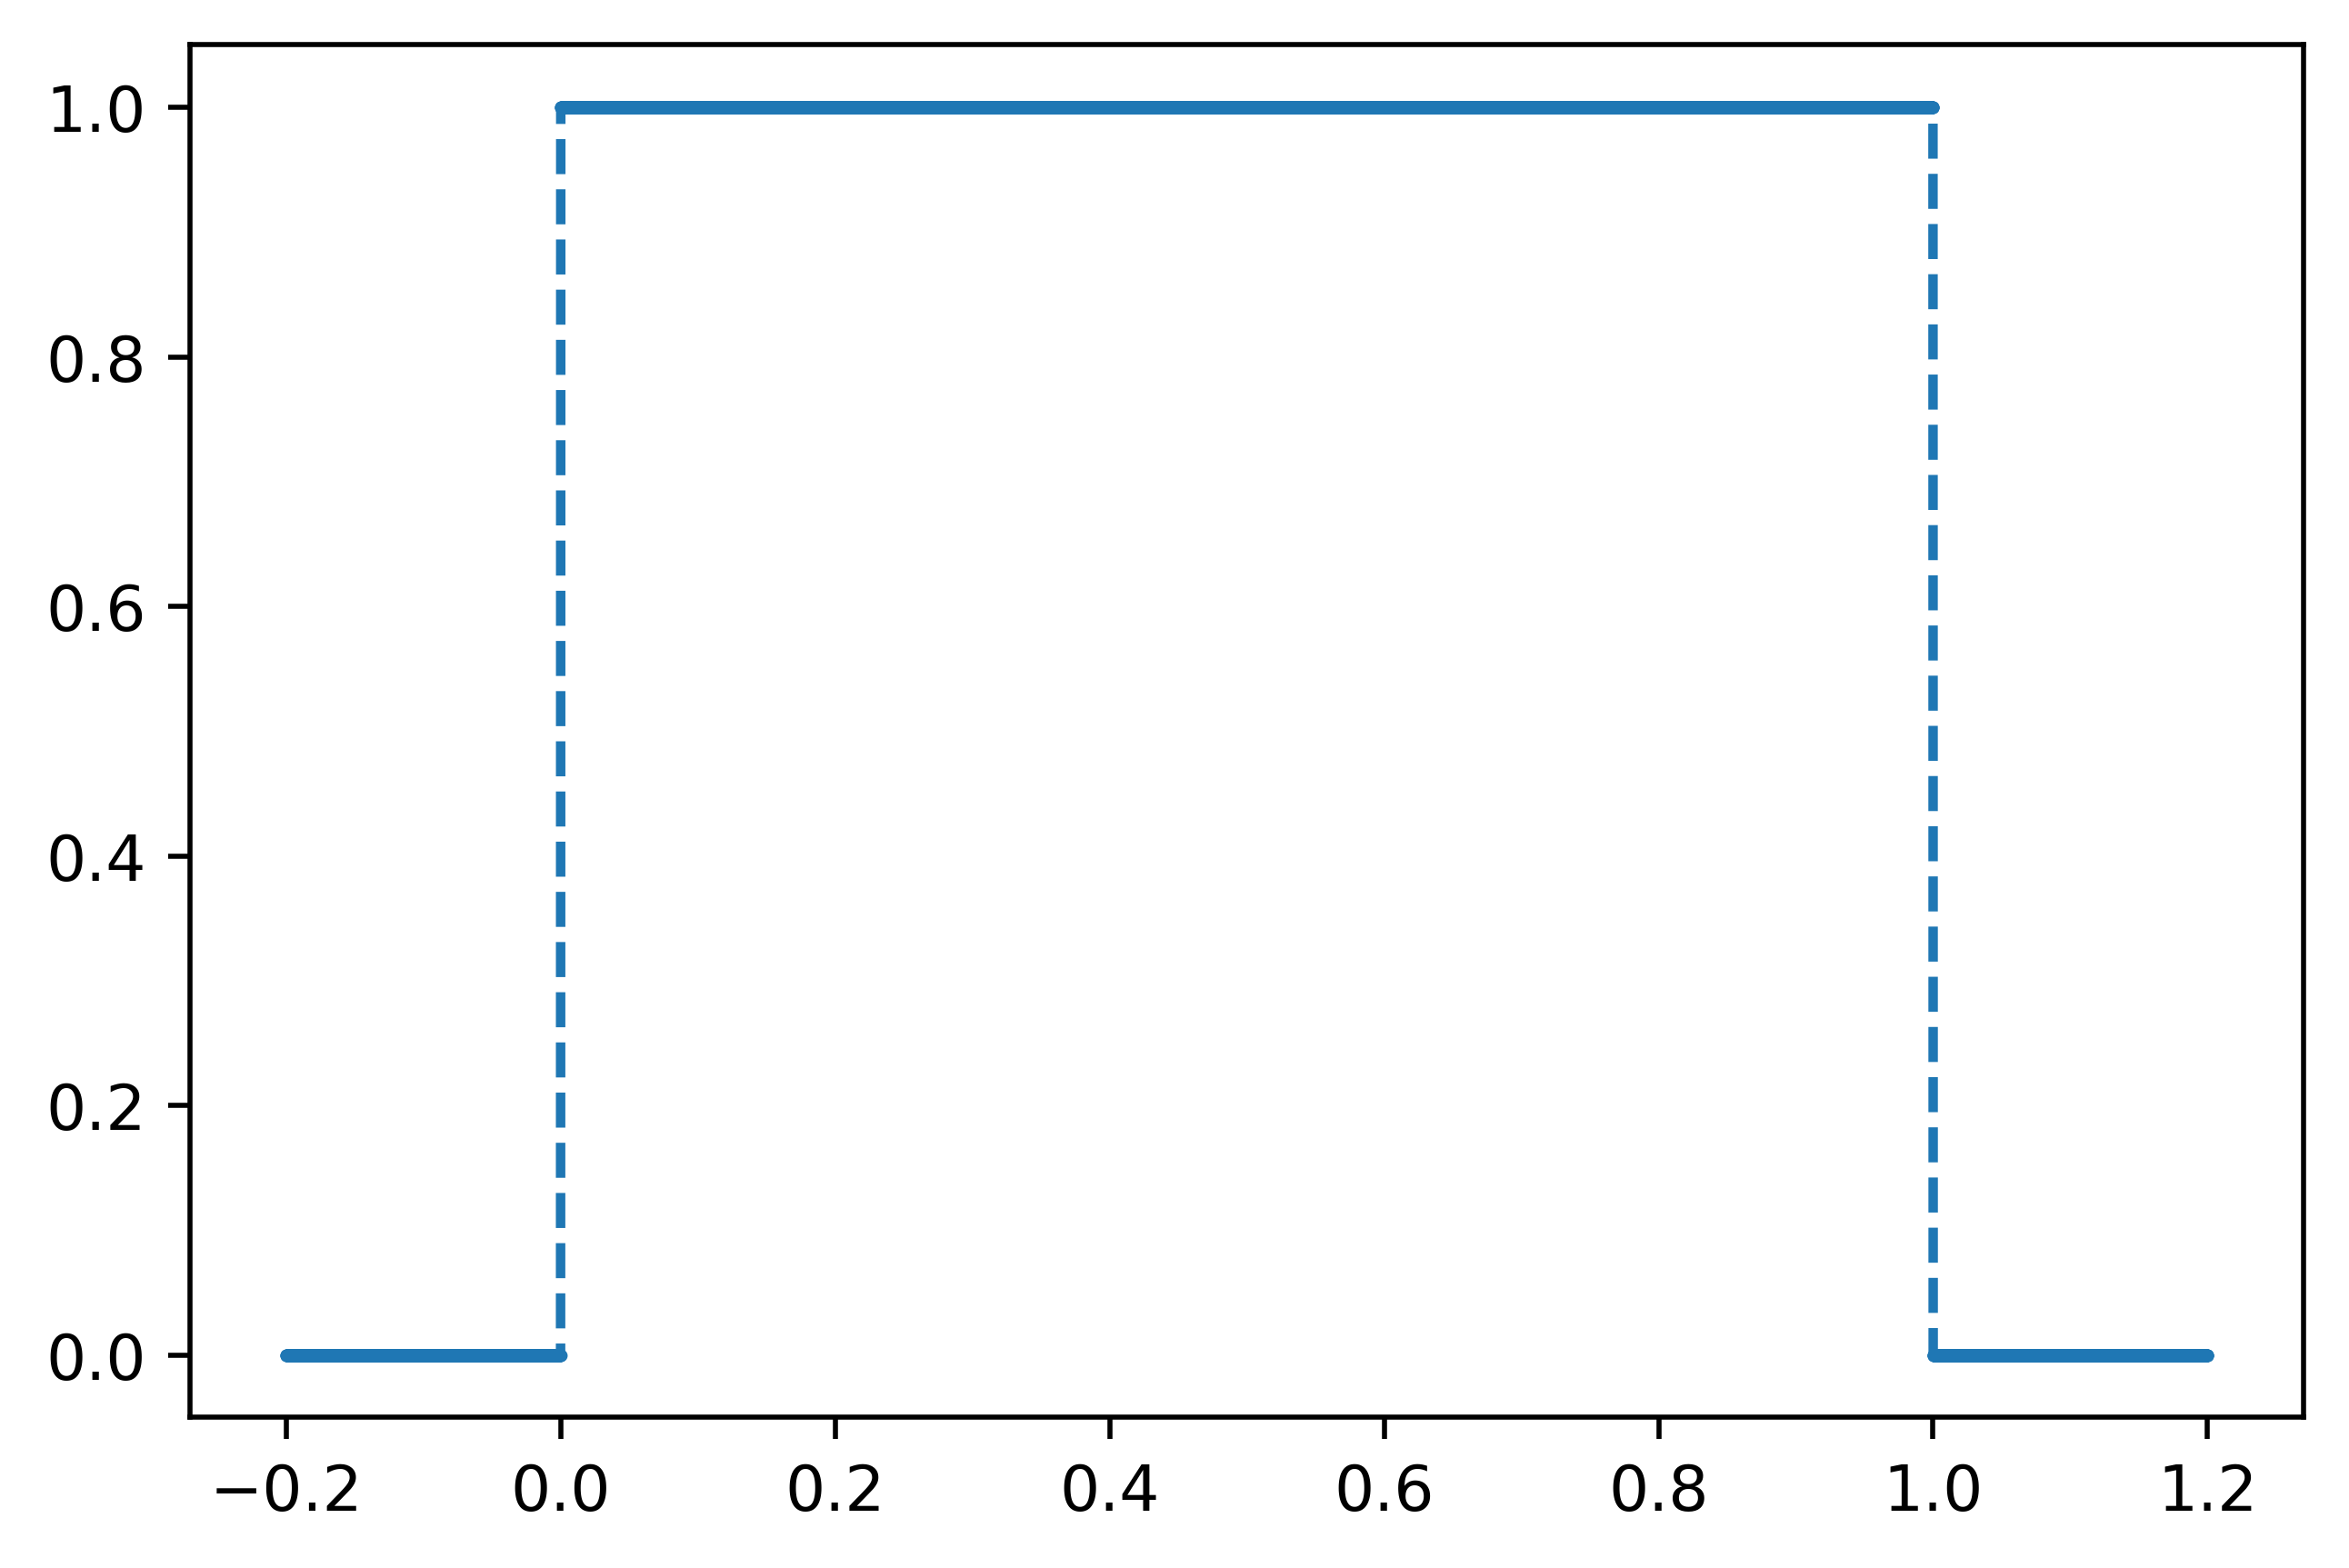
\includegraphics[scale=0.5]{images/uniform.png}
        \caption{PDF of uniform distribution}
        \label{uni_pdf}
    \end{figure}
    \item \textbf{Geometric Distribution}: Unlike the other distributions that we used, this distribution is for a discrete random variable. The PDF is given by
    $$f_X(k) = (1-p)^{k-1}p,\; k=1,2,3,...$$
    In our experiments, we arbitrarily chose to use $p=0.35$. The mean is $\dfrac{1}{p}$ and the standard deviation is $\dfrac{\sqrt{(1-p)}}{p}$. The PMF is given in figure \ref{geom_pmf}. 
    \begin{figure}[H]
        \centering
        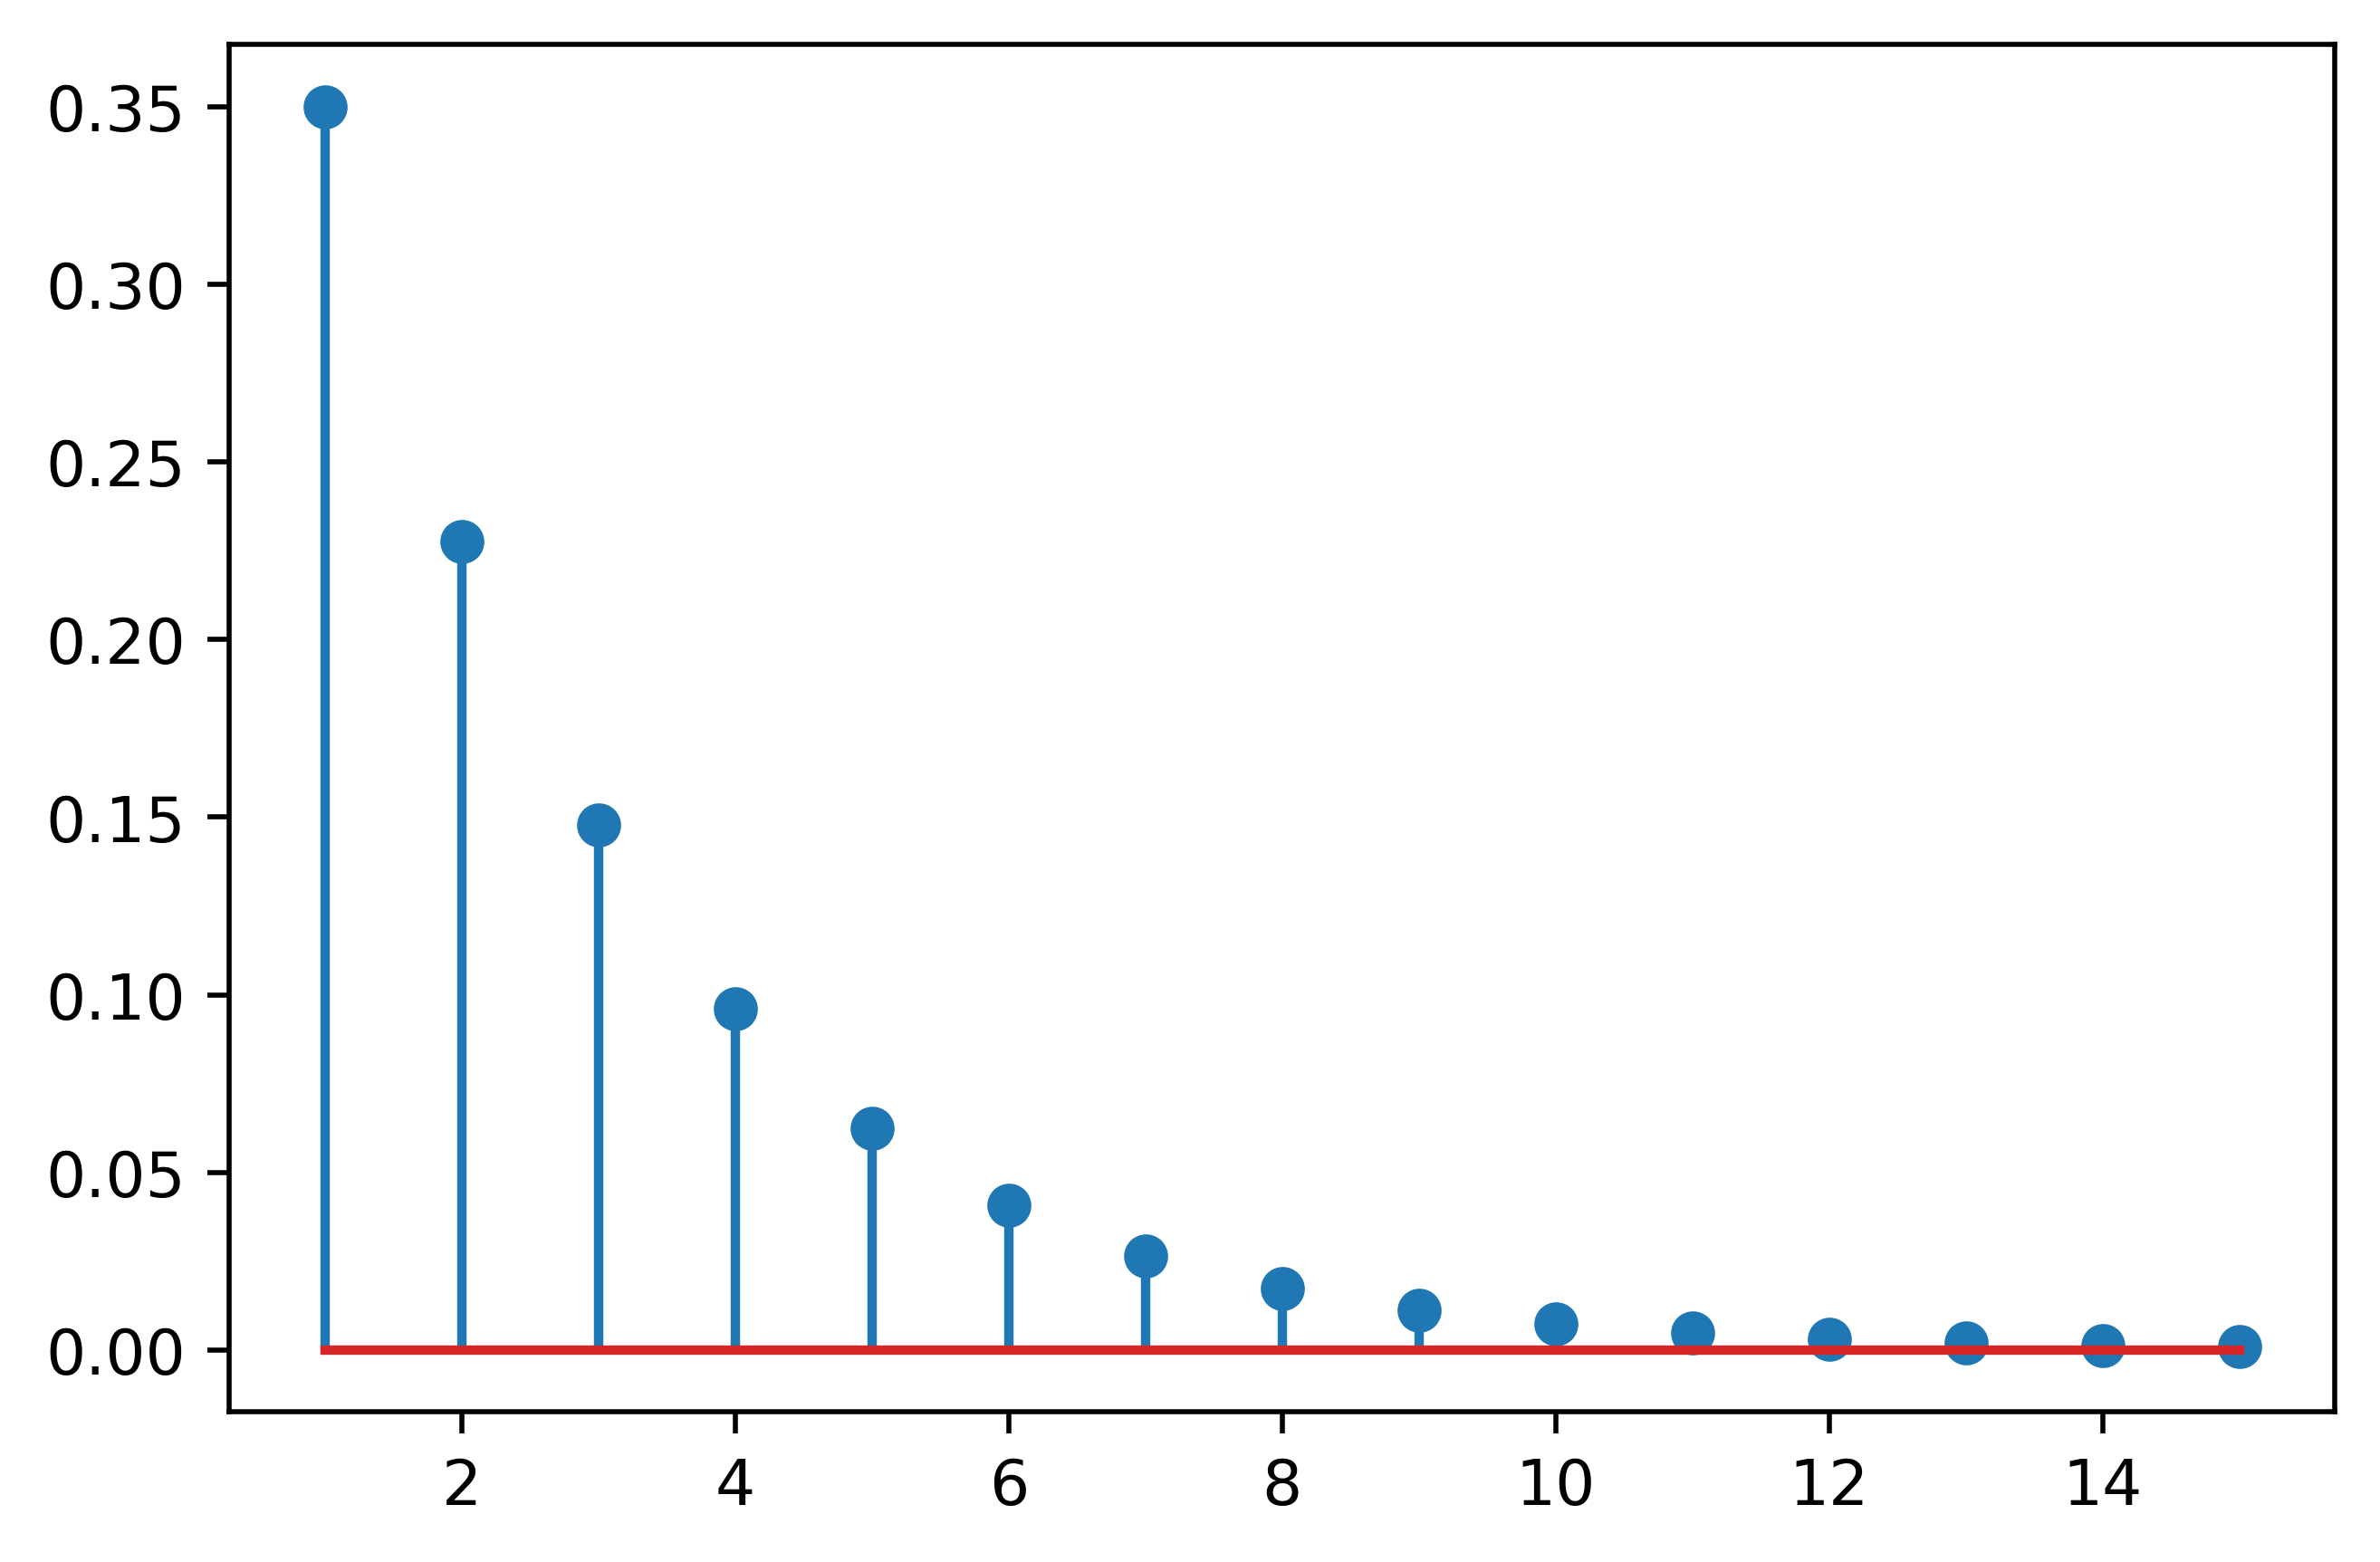
\includegraphics[scale=0.5]{images/geometric.png}
        \caption{PMF of geometric distribution}
        \label{geom_pmf}
    \end{figure}
    \item \textbf{Standard cauchy distribution}: The PDF is given by $$f_X(x) = \dfrac{1}{\pi (1+x^2)}$$ Neither the mean nor the standard deviation are finite. Thus CLT should not apply on this distribution. Figure \ref{cauchy_pdf} shows the PDF of standard cauchy distribution.
    \begin{figure}[H]
        \centering
        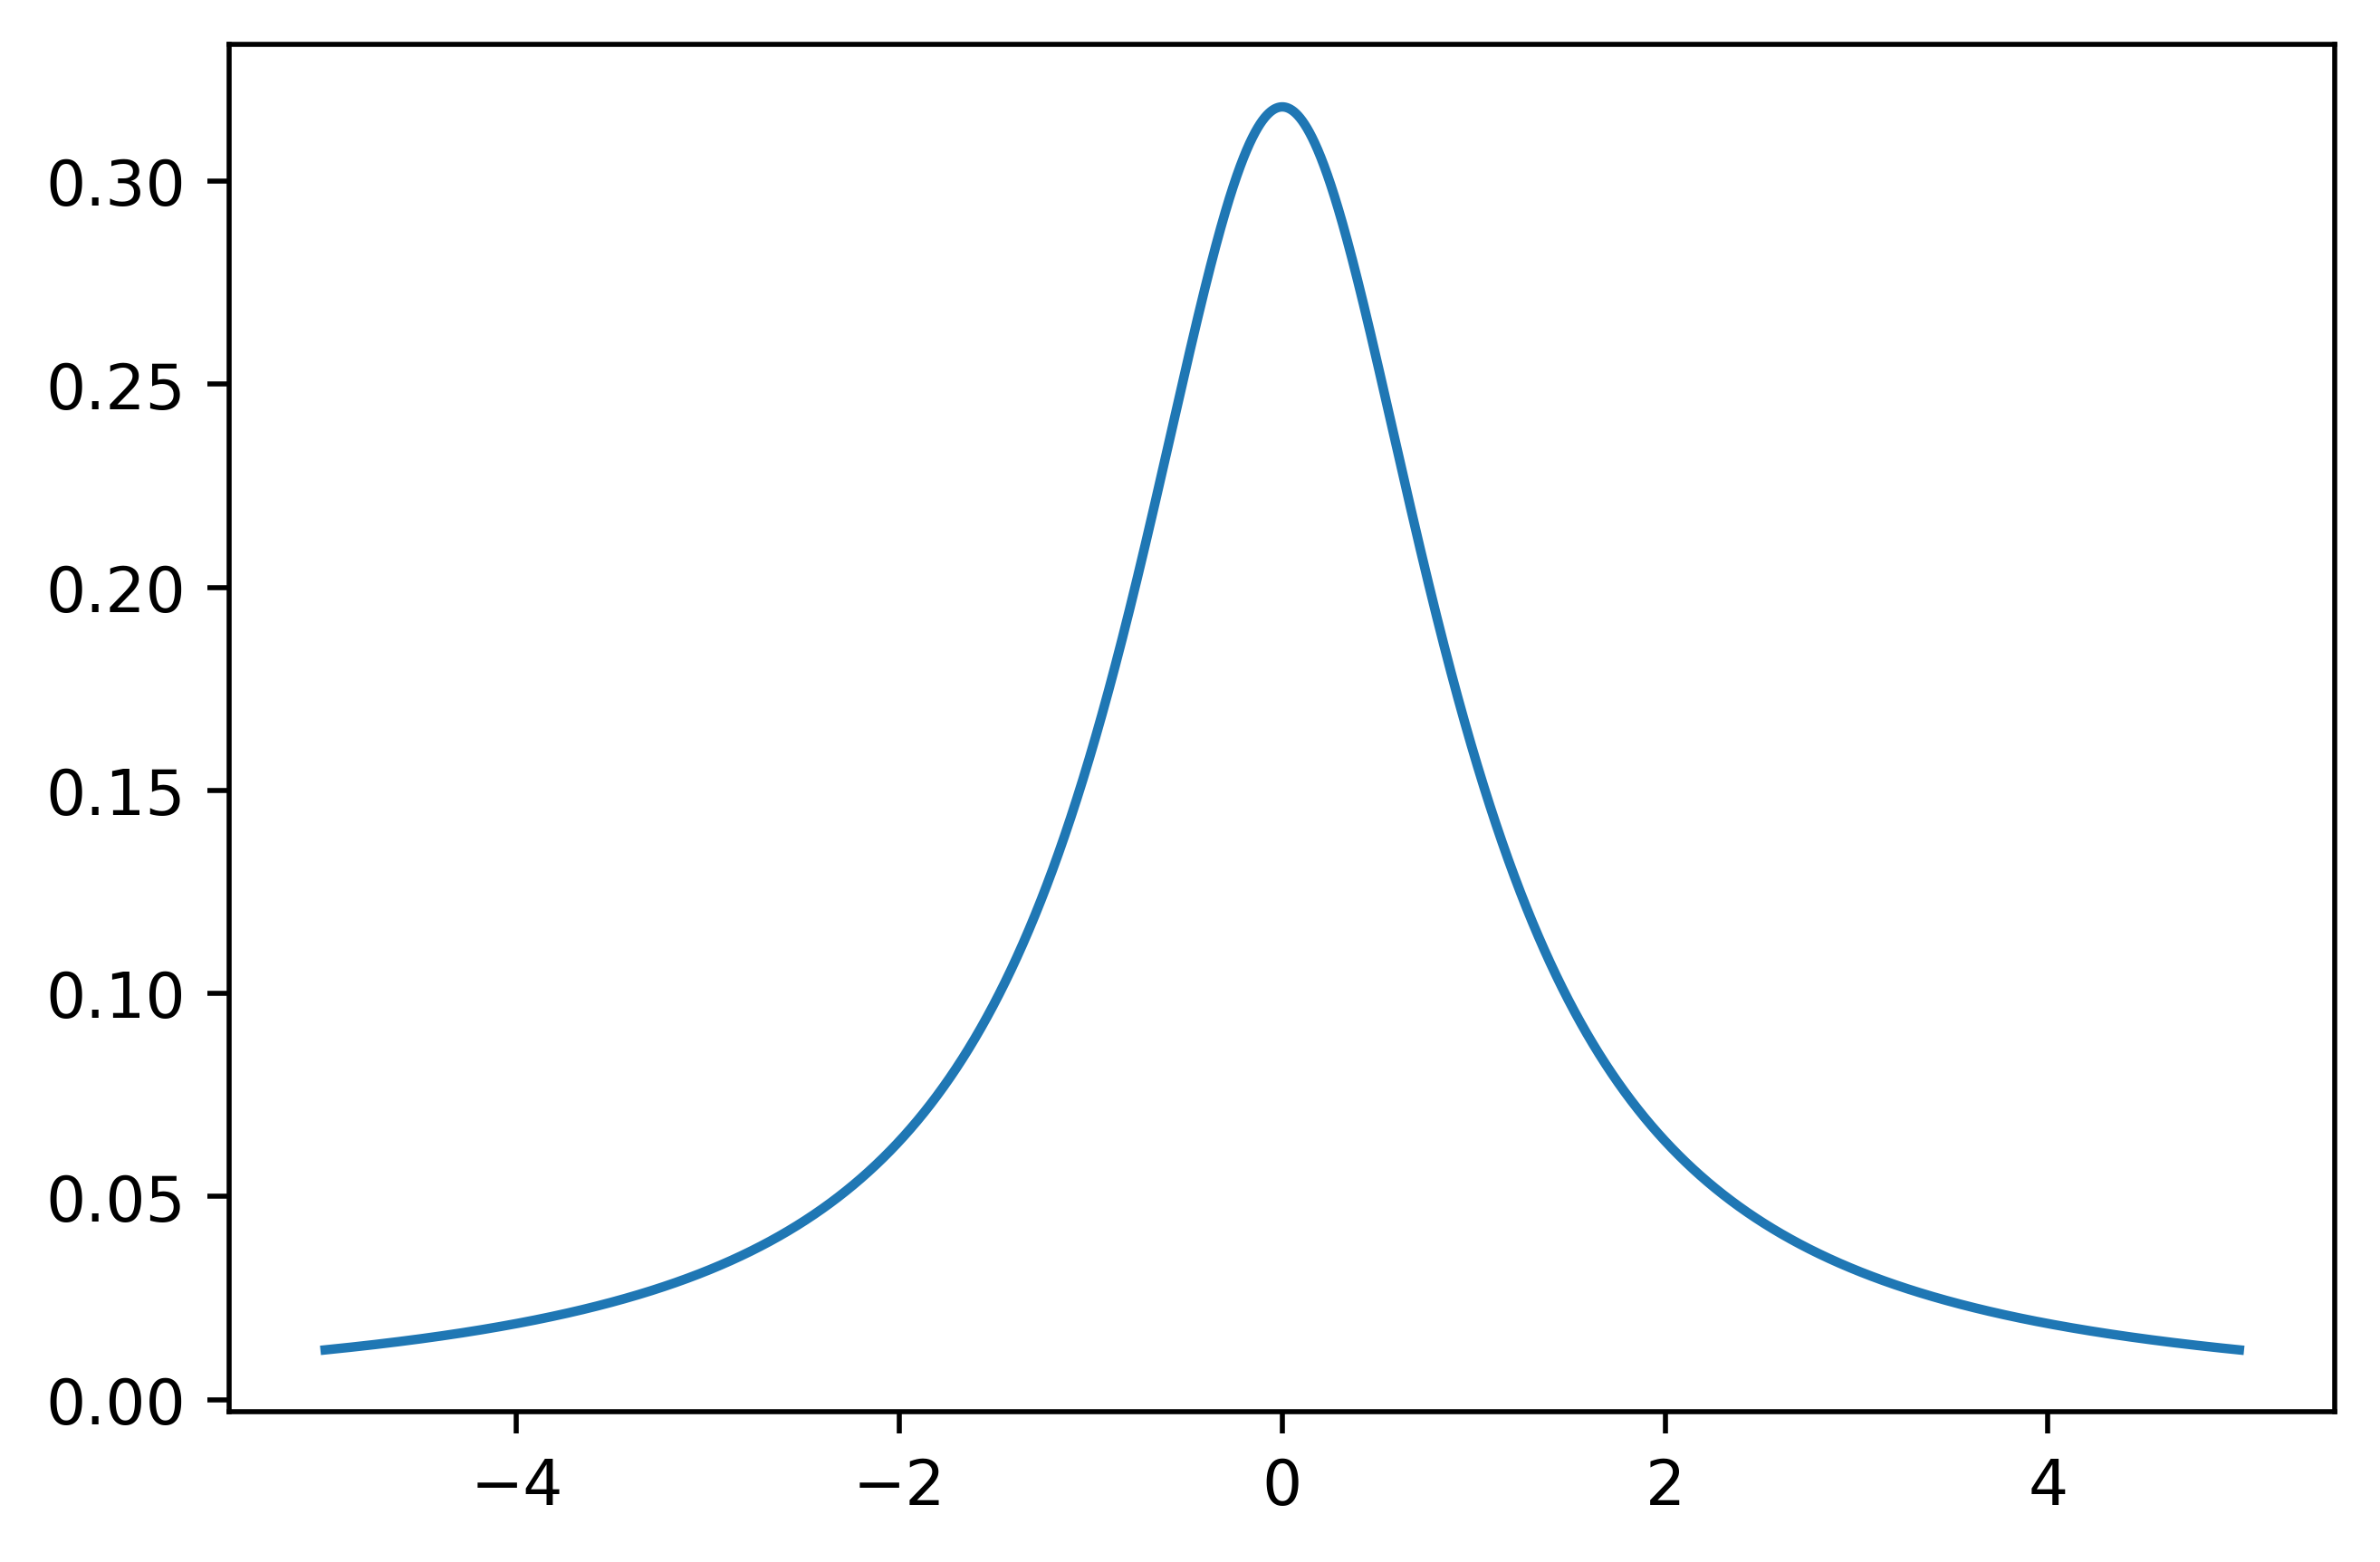
\includegraphics[scale=0.4]{images/cauchy.png}
        \caption{PDF of Cauchy Distribution}
        \label{cauchy_pdf}
    \end{figure}
\end{enumerate}
\section{Shapiro-Wilk Test}

\section{Results}
\section{Conclusion}
\end{document}
